\section{Output Files}
\subsection{Standard ADMB output files}
Standard ADMB files are created by SS. These are:

ss.par – This file has the final parameter values.  They are listed in the order they are declared in SS.  This file can be read back into SS to restart a run with these values (see running SS on page \pageref{sec:RunningSS}).

ss.std – This file has the parameter values and their estimated standard deviation for those parameters that were active during the model run.  It also contains the derived quantities declared as standard deviation report variables.  All of this information is also report in the covar.sso.  Also, the parameter section of Report.sso lists all the parameters with their SS generated names, denotes which were active in the reported run, displays the parameter standard deviations, then displays the derived quantities with their standard deviations.

ss.rep – This report file is created between phases so, unlike Report.sso, will be created even if the hessian fails. It does not contain as much output as shown in Report.sso.

ss.cor – This is the standard ADMB report for parameter and standard deviation report correlations. It is in matrix form and challenging to interpret.  This same information is reported in covar.sso.

\subsection{SS Summary}
The ss\_summary.sso file (available for versions 3.30.08.03 and later) is designed to put key model outputs all in one concise place.  It is organized as a list.  At the top of the file are some descriptors, followed by the likelihoods for each component, then the parameters and their standard errors, then the derived quantities and their standard errors.  The total biomass, summary biomass, and catch were added to the quantities reported in this file in version 3.30.11 and later. This output was created to make it easy to compare the results between different versions of the executable, however, this file could be useful for numerous other uses. 

\subsection{SIS table}
The SIS\_table.sso file contains model output formatted for reading into the NMFS Species Information System (SIS). This file includes an assessment summary for categories of information (abundance, recruitment, spawners, catch estimates) that are input into the SIS database. A time-series of estimated quantities which aggregates estimates across multiple areas and seasons are provided to summarize model results. Access to the SIS database is granted to all NOAA employees and can be accessed as: https://www.st.nmfs.noaa.gov/sis/.

\subsection{Derived Quantities}
Before listing the derived quantities reported to the standard deviation report, there are a couple of topics that deserve further explanation.

\hypertarget{VirginUnfished}{}
\subsubsection{Virgin Spawning Biomass (B0) vs Unfished Spawning Biomass}
Unfished is the condition for which reference points (benchmark) are calculated.  Virgin Spawning Biomass (B0) is the initial condition on which the start of the time-series depends.If biology or SR parameters are time-varying, then the benchmark year input in the forecast file tells SS which years to average in order to calculate "unfished". In this case, virgin recruitment and/or the virgin spawning biomass will differ from their unfished counterparts. Virgin recruitment and spawning biomass are reported in the mgmt\_quant portion of the sd\_report and are now labeled as "unfished" for clarity.  Note that if ln(R0) is time-varying, then this will cause unfished to differ from virgin. However, if regime shift parameter is time-varying, then unfished will remain the same as virgin because the regime shift is treated as a temporary offset from virgin. Virgin spawning biomass is denoted as SPB\_virgin and spawning biomass unfished is denoted as SPB\_unf in the report file.

Virgin Spawning Biomass (B0) is used in four ways within SS:
\begin{enumerate}
	\item Anchor for the spawner-recruitment relationship as virgin spawning biomass.
	\item Basis for the initial equilibrium abundance. 
	\item Basis against which annual depletion is calculated.
	\item Benchmark calculations.
\end{enumerate}
However, if there is time-varying biology, then the 4th usage can have a different B0 calculation compared to the other usages.

\subsubsection{Metric for Fishing Mortality}
A generic single metric of annual fishing mortality is difficult to define in a generalized model that admits multiple areas, multiple biological cohorts, dome-shaped selectivity in size and age for each of many fleets. Several separate indices are provided and others could be calculated by a user from the detailed information in Report.sso.

\subsubsection{Equilibrium SPR}
This index focuses on the effect of fishing on the spawning potential of the stock. It is calculated as the ratio of the equilibrium reproductive output per recruit that would occur with the current year's F intensities and biology, to the equilibrium reproductive output per recruit that would occur with the current year's biology and no fishing.  Thus it internalizes all seasonality, movement, weird selectivity patterns, and other factors. Because this index moves in the opposite direction than F intensity itself, it is usually reported as 1-SPR. A benefit of this index is that it is a direct measure of common proxies used for F\textsubscript{MSY}, such as F\textsubscript {40\%}. A shortcoming of this index is that it does not directly demonstrate the fraction of the stock that is caught each year. The SPR value is also calculated in the benchmarks (see below). 

The derived quantities report shows an annual SPR statistic.  The options, as specified in the starter.ss file, are:
\begin{itemize}
	\item 0 = skip
	\item 1 = (1-SPR)/(1-SPR\textsubscript{TGT})
	\item 2 = (1-SPR)/(1-SPR\textsubscript{MSY})
	\item 3 = (1-SPR)/(1-SPR\textsubscript{Btarget})
	\item 4 = raw SPR
\end{itemize}

The SPR approach to measuring fishing intensity was implemented because the concept of a single annual F does not exist in SS because F varies by age, sex, and growth morph and season and area.  There is no single F value that is applied to all ages unless you create a very simple SS setup with knife-edge selectivity.  So, what you see in the SS options are various ways to calculate annual fishing intensity.  They can be broken down into three categories.  One is exploitation rate calculated simply as total catch divided by biomass from a defined age range. Another is SPR, which is a single measure of the equilibrium effect of fishing according to the F.  The third category are various ways to calculate an average F. Some measures of fishing intensity will be misleading if applied inappropriately. For example, the sum of the apical F's will be misleading if different fleets have very different selectivities or, worse, if they occur in different areas. The F=Z-M approach to getting fishing intensity is a way to have a single F that represents a number's weighted value across multiple areas, sexes, morphs, ages. An important distinction is that the exploitation rate and F-based approaches directly relate to the fraction of the population removed each year by fishing; whereas the SPR approach represents the cumulative effect of fishing so it's equivalent in F-space depends on M.

\subsubsection{F std}
This index provides a direct measure of fishing mortality.  The options are:
\begin{itemize}
	\item 0 = skip
	\item 1 = exploitation(Bio)
	\item 2 = exploitation(Num)
	\item 3 = sum(Frates)
\end{itemize}
The exploitation rates are calculated as the ratio of the total annual catch (in either biomass or numbers as specified) to the summary biomass or summary numbers on January 1.  The sum of the F rates is simply the sum of all the apical Fs.  This makes sense if the F method is in terms of instantaneous F (not Pope's approximation) and if there are not fleets with widely different size/age at peak selectivity, and if there is no seasonality, and especially if there is only one area.  In the derived quantities, there is an annual statistic that is the ratio of the can be annual F\_std value to the corresponding benchmark statistic.  The available options for the denominator are:
\begin{itemize}
	\item 0 = raw
	\item 1 = F/F\textsubscript {SPR}
	\item 2 = F/F\textsubscript {MSY}
	\item 3 = F/F\textsubscript {Btarget}
\end{itemize}

\subsubsection{F-at-Age}
Because the annual F is so difficult to interpret as a sum of individual F components, an indirect calculation of F-at-age is reported at the end of the report.sso file. This section of the report calculates Z-at-age simply as $ln(N_{a+1,t+1}/N_{a,t})$. This is done on an annual basis and summed over all areas. It is done once using the fishing intensities as estimated (to get Z), and once with the F intensities set to 0.0 to get M-at-age. This latter sequence also provides a measure of dynamic Bzero.  The user can then subtract the table of M-at-age/year from the table of Z-at-age/year to get a table of F-at-age/year. From this apical F, average F over a range of ages, or other user-desired statistics could be calculated.  urther work within SS with this table of values is anticipated.

\subsubsection{MSY and other Benchmark Items}
The following quantities are included in the sdreport vector mgmt\_quantities, so obtain estimates of variance.  Some additional quantities can be found in the benchmarks section of the forecast\_report.sso.

\begin{center}
	\begin{longtable}{p{4cm} p{11cm}}
		\hline
		Benchmark Item &  Description\Tstrut\Bstrut\\
		\hline
		\endfirsthead

		\hline
		Benchmark Item &  Description\Tstrut\Bstrut\\
		\hline
		\endhead
		
		\endfoot
		\hline		
		\endlastfoot
		
		SSB\_Unfished \Tstrut& Unfished reproductive potential (SSB is commonly female mature spawning biomass).\\
		TotBio\_Unfished \Tstrut& Total age 0+ biomass on January 1.\\
		SmryBio\_Unfished \Tstrut& Biomass for ages at or above the summary age on January 1.\\
		Recr\_Unfished \Tstrut& Unfished recruitment.\\
		SSB\_Btgt \Tstrut& SSB at user specified SSB target.\\
		SPR\_Btgt \Tstrut& Spawner potential ratio (SPR) at F intensity that produces user specified SSB target.\\
		Fstd\_Btgt \Tstrut& F statistic at F intensity that produces user specified SSB target.\\
		TotYield\_Btgt \Tstrut& Total yield at F intensity that produces user specified SSB target.\\
		SSB\_SPRtgt \Tstrut& SSB at user specified SPR target (but taking into account the spawner-recruitment relationship).\\
		Fstd\_SPRtgt \Tstrut& F intensity that produces user specified SPR target.\\
		TotYield\_SPRtgt \Tstrut& Total yield at F intensity that produces user specified SPR target.\\
		SSB\_MSY \Tstrut& SSB at F intensity that is associated with MSY; this F intensity may be directly calculated to produce MSY, or can be mapped to F\_SPR or F\_Btgt.\\
		SPR\_MSY \Tstrut& Spawner potential ratio (SPR) at F intensity associated with MSY.\\
		Fstd\_MSY \Tstrut& F statistic at F intensity associated with MSY.\\
		TotYield\_MSY \Tstrut& Total yield (biomass) at MSY.\\
		RetYield\_MSY \Tstrut& Retained yield (biomass) at MSY.\Bstrut\\ 
	\end{longtable}
\end{center}

\subsection{Brief cumulative output}
Cum\_Report.sso: contains a brief version of the run output, which is appended to current content of file so results of several runs can be collected together. This is especially useful when a batch of runs is being processed. Unless this file is deleted, it will contain a cumulative record of all runs done in that subdirectory. The first column contains the run number.  

\hypertarget{bootstrap}{}
\subsection{Bootstrap Data Files}
It is possible to create bootstrap data files for SS where an internal parametric bootstrap function generates a simulated data set by parametric bootstrap sampling the expected values given the input observation error. The number of bootstrap data files to create is specified in the starter file where a value of 3 or greater will create a single bootstrap data file in the data.ss\_new file. The first output provides the unaltered input data file (with annotations added).  The second provides the expected values for only the data elements used in the model run.  The third and subsequent outputs provide parametric bootstraps around the expected values. The bootstrap data file can be parsed using r4ss function SS\_splitdat into individual data files and re-run with the model.

The bootstrapping procedure within SS is done via the following steps:

\begin{itemize}
	\item Expected values of all input data are calculated (these are also used in the likelihood which compares observed to expected values for all data). The calculation of these expected values is described in detail under the "Observation Model" section of the appendix to \citet{methot_stock_2013}. \
	
	\item Parametric bootstrap data are calculated for each observation by sampling from a probability distribution corresponding to the likelihood for that data type using the expected values noted above. Examples of how this happens include the following:
	
	\begin{itemize}
		\item Indices of abundance are sampled from the distribution used in the estimation model (as set in the “Errtype” column of the index configuration, most commonly lognormal but could be normal or T-distribution). The variability of the distribution from which the random sample is drawn is based on the combination of the input uncertainty and any estimated "Extra SD" parameter and any "add\_to\_survey\_CV" value included under the input variance adjustments factors.
		
		\item Length and age compositions are sampled from multinomial distributions with expected proportions in each bin based on the expected values and sample size equal to the adjusted input sample size (input sample size multiplied by any inputs for "mult\_by\_lencomp\_N" or "mult\_by\_agecomp\_N" under the input variance adjustments factors).
		
		\item Discard data (fractions or absolute amounts) are generated from the chosen distribution (T-distribution, normal, log-normal, truncated-normal).
		
		\item Tagging data is generated using a negative binomial distribution to get the total number of recaptures for each tag group and a multinomial distribution to allocate those recaptures among fleets.
	\end{itemize}
\end{itemize}

Given this, there are some assumptions implicit in the bootstrapping procedure (as implemented as of v.3.30.14) that users should be aware of:

\begin{itemize}
	\item This procedure is strictly an observation error approach (i.e., process error in recruitment or any other time-varying parameter is not added). For simulation analyses, a common approach has been to input a new time series of recruitment deviations for each bootstrap data set.
	
	\item The sample size for conditional age-at-length data matches the inputs for each length bin. If stratified sampling is used, this may be appropriate, but if the ages represent a random subset of the selected population, this may result in less variability than if the associated length distribution were resampled.
	
	\item Currently, the aging error matrix is multiplied by the expected distribution of proportions at age, while the more correct order of operations would be to sample true ages, and then sample the observed age including aging error (it is possible these are mathematically identical).
	
	\item Often there is need to explore the removal (not include in the model fitting) of specific years in a data set which can be done by specifying a negative fleet number. If bootstrapping a data file, note that specifying a negative fleet in the data inputs for indices, length composition, or age composition will include the "observation" in the model (hence generating predicted values and bootstrap data sets for the data), but not in the negative log likelihood. The "observation values" used with negative fleet do not influence the predicted values, except when using tail compression with length or age composition. Non-zero values greater than the minimum tail compression should be used for the observation values when tail compression is being used, as using zeros or values smaller than the minimum tail compression can cause the predicted values to be reported as zero and shift predictions to other bins.
\end{itemize}

\subsection{Forecast and Reference Points (Forecast-report.sso)}
The Forecast-report file contains output of fishery reference points and forecasts.  It is designed to meet the needs of the Pacific Fishery Management Council's Groundfish Fishery Management Plan, but it should be quite feasible to develop other regionally specific variants of this output.

The vector of forecast recruitment deviations is estimated during an additional model estimation phase.  This vector includes any years after the end of the recruitment deviation time series and before or at the end year. When this vector starts before the ending year of the time series, then the estimates of these recruitments will be influenced by the data in these final years. This is problematic, because the original reason for not estimating these recruitments at the end of the time series was the poor signal/noise ratio in the available data. It is not that these data are worse than data from earlier in the time series, but the low amount of data accumulated for each cohort allows an individual datum to dominate the model's fit. Thus, an additional control is provided so that forecast recruitment deviations during these years can receive an extra weighting in order to counter-balance the influence of noisy data at the end of the time series.

An additional control is provided for the fraction of the log-bias adjustment to apply to the forecast recruitments. Recall that R is the expected mean level of recruitment for a particular year as specified by the spawner-recruitment curve and R' is the geometric mean recruitment level calculated by discounting R with the log-bias correction factor $e-0.5s^2$. Thus a lognormal distribution of recruitment deviations centered on R' will produce a mean level of recruitment equal to R. During the modeled time series, the virgin recruitment level and any recruitments prior to the first year of recruitment deviations are set at the level of R, and the lognormal recruitment deviations are centered on the R' level.  For the forecast recruitments, the fraction control can be set to 1.0 so that 100\% of the log-bias correction is applied and the forecast recruitment deviations will be based on the R' level. This is certainly the configuration to use when the model is in MCMC mode. Setting the fraction to 0.0 during maximum likelihood forecasts would center the recruitment deviations, which all have a value of 0.0 in maximum likelihood mode, on R. Thus would provide a mean forecast that would be more comparable to the mean of the ensemble of forecasts produced in MCMC mode.  Further work on this topic is underway.

Note:
\begin{itemize}
	\item Cohorts continue growing according to their specific growth parameters in the forecast period rather than staying static at the end year values.
	\item Environmental data entered for future years can be used to adjust expected recruitment levels.  However, environmental data will not affect growth or selectivity parameters in the forecast.
\end{itemize}

The top of the Forecast-report file shows the search for F\textsubscript {SPR}  and the search for F\textsubscript {MSY}, allowing the user to verify convergence. Note: if the STD file shows aberrant results, such as all the standard deviations being the same value for all recruitments, then check the F\textsubscript {MSY} search for convergence. The F\textsubscript {MSY} can be calculated, or set equal to one of the other F reference points per the selection made in starter.ss.

%The reference point output is shown in the the table below: 
%\begin{center}
%	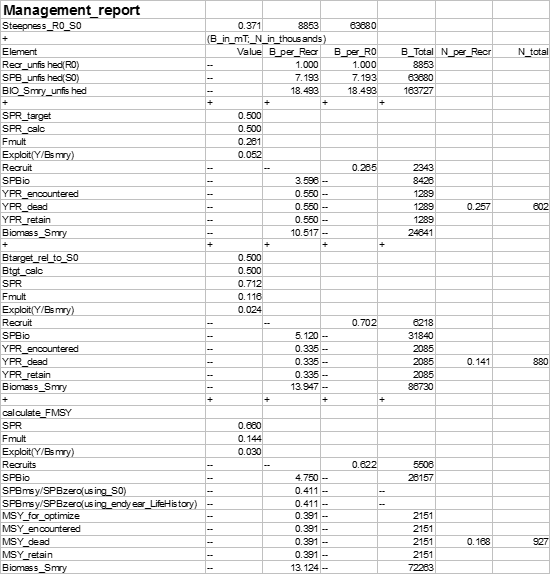
\includegraphics{ManagementReport}
%\end{center}


%\begin{landscape}
%The forecast is done once using the Target SPR and once using the adjustments specified in the 40:10 section of forecast.ss input. Each section contains a time series of seasonal biomass and catch, followed by a time series of population numbers-at-age for each platoon.
	
%	\begin{center}
%		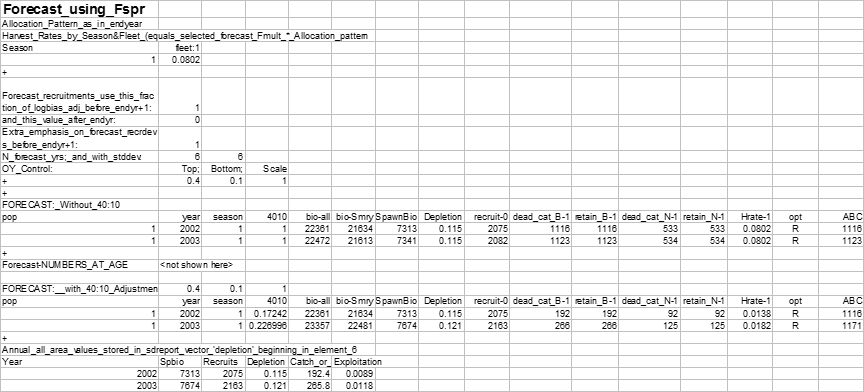
\includegraphics{Forecast}
%	\end{center}
%\end{landscape}

%where:
%\begin{itemize}
%	\item 40:10 is the magnitude of the adjustment of harvest multiplier to implement the optimum yield policy;
%	\item bio-all is the biomass of all ages;
%	\item bio-smry is the biomass for ages at or above the summary age;
%	\item Spawnbio - is the female spawning biomass/output;
%	\item Depletion is the spawning biomass/output divided by the unfished spawning biomass/output;
%	\item Recruit-0 is the recruitment of age-o fish in this year;
%	\item Dead\_cat\_B-1 is the total dead (retained plus dead discard) catch in MT for fleet 1;
%	\item Retain\_B-1 is fleet 1's retained catch in MT;
%	\item Equivalent catch in numbers is then reported;
%	\item Hrate-1 is the harvest rate, as adjusted by the 40:10 policy.  The units will depend on the F method selected (Pope's method giving mid-year harvest rate or the continuous F).
%	\item Opt=C means that the rate was calculated from an input catch level (and crashed means that this caused an excessive harvest rate.
%	\item Opt=R means that the catch was calculated from the target harvest rate.; and
%	\item ABC is equal to the Total-Catch when the 40:10 option is not used (upper portion of table).  When the 40:10 is on (lower table), the ABC is the catch level corresponding to no 40:10 adjustment after accounting for catch in previous year's from the 40:10.
%\end{itemize}

%The time series output described above is detailed by season, area, platoon and fishery.  It is usually more convenient to have annual values summed across areas, platoons and fisheries.  This is done for the 40:10 output and a subset of these values are replicated in the depletion vector in the sd\_report so that variance estimates can be obtained.  The elements of the depletion vector in the sd\_report are:
%\begin{itemize}
%	\item depletion level in end year
%	\item depletion level in end year+1
%	\item MSY (if calculated, else spbio in endyr-1)
%	\item B\textsubscript{MSY} (if calculated, else spbio in endyr)
%	\item SPR\textsubscript{MSY} (if calculated, else spbio in endyr+1) then the time series of:
%	\begin{itemize}
%		\item Spawning biomass
%		\item Recruitment
%		\item Depletion level
%		\item Total catch (if forecast calculated catch from rates) or sum of fishery-specific harvest rates (if forecast is based on fixed input catch level in this year)
%		\item Total exploitation rate (total dead catch divided by the summary biomass at the beginning of the year).
%	\end{itemize}
%\end{itemize}

%\begin{center}
%	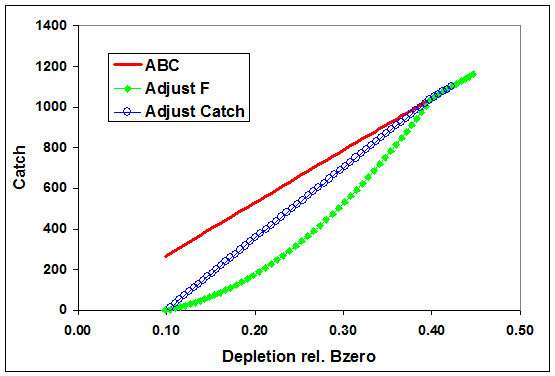
\includegraphics{HCR}\\
%	Two examples of harvest forecast adjustment: one adjusts catch and the other adjusts F.
%\end{center}

\subsection{Main Output File, Report.sso}
This is the primary output file.  Its major sections are listed below.  

The sections of the output file are:
\begin{itemize}
	\item SS version number with date compiled.  Time and date of model run.  This info appears at the top of all output files.
	\item Comments
		\begin{itemize}
			\item 	Input file lines starting with \#C are echoed here.
		\end{itemize}
	\item Keywords
		\begin{itemize}
			\item List of keywords used in searching for output sections.
		\end{itemize}
	\item Fleet Names
		\begin{itemize}
			\item List of fishing fleet and survey names assigned in the data file.
		\end{itemize}
	\item Likelihood
		\begin{itemize}
			\item Final values of the negative log(likelihood) are presented.
		\end{itemize}
	\item Input Variance Adjustments
		\begin{itemize}
			\item The matrix of input variance adjustments is output here because these values affect the log likelihood calculations.
		\end{itemize}
	\item Parameters
		\begin{itemize}
			\item The parameters are listed here.  For the estimated parameters, the display shows: Num (count of parameters), Label (as internally generated by SS), Value, Active\_Cnt, Phase, Min, Max, Init, Prior, Prior\_type, Prior\_SD, Prior\_Like, Parm\_StD (standard deviation of parameter as calculated from inverse Hessian), Status (e.g. near bound), and Pr\_atMin (value of prior penalty if parameter was near bound).  The Active\_Cnt entry is a count of the parameters in the same order they appear in the ss.cor file.
		\end{itemize}
	\item Derived Quantities
		\begin{itemize}
			\item This section starts by showing the options selected from the starter.ss and forecast.ss input files:
				\begin{itemize}
					\item SPR ratio basis
					\item F report basis
					\item B ratio denominator
				\end{itemize}
		\end{itemize}
\end{itemize}

Then the time series of output, with standard deviation of estimates, are produced with internally generated labels.  Note that these time series extend through the forecast era.  The order of the output is: spawning biomass, recruitment, SPRratio, Fratio, Bratio, management quantities, forecast catch (as a target level), forecast catch as a limit level (OFL), Selex\_std, Grow\_std, NatAge\_std.  For the three "ratio" quantities, there is an additional column of output showing a Z-score calculation of the probability that the ratio differs from 1.0. The "management quantities" section is designed to meet the terms of reference for west coast groundfish assessments; other formats could be made available upon request. The standard deviation quantities at the end are set up according to specifications at the end of the control input file. In some cases, a user may specify that no derived quantity output of a certain type be produced. In those cases, SS substitutes a repeat output of the virgin spawning biomass so that vectors of null length are not created.

ADMB note, while vectors of null length are very useful for controlling optional model inputs, they cannot be used with current version of ADMB for sdreport quantities.

\begin{itemize}
	\item Mortality-growth parameter by year after adjustments
	\begin{itemize}
		\item This block shows the time series of mortality-growth parameters by year after adjustment by environmental links, blocks and deviations.
	\end{itemize}
	\item Selectivity parameters (size) by year after adjustments
	\begin{itemize}
		\item This block shows the size selectivity parameters, after adjustment, for each year in which a change occurs.
	\end{itemize}
	\item Selectivity parameters (age) by year after adjustments
	\begin{itemize}
		\item This block shows the age selectivity parameters, after adjustment, for each year in which a change occurs.
	\end{itemize}
	\item Recruitment Distribution
	\begin{itemize}
		\item This block shows the distribution of recruitment across growth patterns, genders, birth seasons, and areas in the end year of the model.
	\end{itemize}
	\item Platoon Indexing
	\begin{itemize}
		\item This block shows the internal index values for various quantities.  It can be a useful reference for complex model setups. The vocabulary is: Bio\_Pattern refers to a collection of cohorts with the same defined growth and natural mortality parameters; sex is the next main index. If recruitment occurs in multiple seasons, then birth season is the index for that factor. The index labeled "Platoon" is used as a continuous index across all the other factor-specific indices. If sub-platoons are used, they are nested within the Bio\_Pattern x Sex x Birth Season platoon. However, some of the output tables use the column label "platoon" as a continuous index across platoons and sub-platoons. Note that there is no index here for area. Each of the cohorts is distributed across areas and they retain their biological characteristics as they move among areas.
	\end{itemize}
	\item Size Frequency Translation
	\begin{itemize}
		\item If the generalized size frequency approach is used, this block shows the translation probabilities between population length bins and the units of the defined size frequency method.  If the method uses body weight as the accumulator, then output is in corresponding units.
	\end{itemize}
	\item Movement
	\begin{itemize}
		\item This block shows movement rate between areas in a multi-area model.
	\end{itemize}
	\item Exploitation
	\begin{itemize}
		\item This block shows the time series of the selected F\_std unit and the F multiplier for each fleet in terms of harvest rate (if Pope's approximation is used) or fully selected F.
	\end{itemize}
	\item Index 2
	\begin{itemize}
		\item This section reports the observed and expected values for each index. All are reported in one list with index number included as a selection field. At the bottom of this section, the root mean squared error of the fit to each index is compared to the mean input error level to assist the user in gauging the goodness-of-fit and potentially adjusting the input level of imprecision.
	\end{itemize}
	\item Index 3
	\begin{itemize}
		\item This section shows the parameter number assigned to each parameter used in this section.
	\end{itemize}
	\item Discard
	\begin{itemize}
		\item This is the list of observed and expected values for the amount (or fraction) discard.
	\end{itemize}
	\item Mean Body Wt
	\begin{itemize}
		\item This is the list of observed and expected values for the mean body weight.
	\end{itemize}
	\item Fit Len Comps
	\begin{itemize}
		\item This is the list of the goodness of fit to the length compositions. The input and output levels of effective sample size are shown as a guide to adjusting the input levels to better match the model's ability to replicate these observations.
	\end{itemize}
	\item Fit Age Comps
	\begin{itemize}
		\item This has the same format as the length composition section.
	\end{itemize}
	\item Fit Size Comps
	\begin{itemize}
		\item This has the same format as the length composition section and is used for the generalized size composition summary.
	\end{itemize}
	\item Len Selex
	\begin{itemize}
		\item Here is the length selectivity and other length specific quantities for each fishery and survey.
	\end{itemize}
	\item Age Selex
	\begin{itemize}
		\item Here is reported the time series of age selectivity and other age-related quantities for each fishery and survey. Some are directly computed in terms of age, and others are derived from the combination of a length-based factor and the distribution of size-at-age.
	\end{itemize}
	\item Environmental Data
	\begin{itemize}
		\item The input values of environmental data are echoed here. In the future, the summary biomass in the previous year will be mirrored into environmental column –2 and that the age zero recruitment deviation into environmental column –1. Once so mirrored, they may enable density-dependent effects on model parameters.
	\end{itemize}
	\item Numbers at Age
	\begin{itemize}
		\item The output (in thousands of fish) is shown for each cohort tracked in the model.
	\end{itemize}
	\item Numbers at Length
	\begin{itemize}
		\item The output is shown for each cohort tracked in the model.
	\end{itemize}
	\item Catch at Age
	\begin{itemize}
		\item The output is shown for each fleet.  It is not necessary to show by area because each fleet operates in only one area.
	\end{itemize}
	\item Biology
	\begin{itemize}
		\item The first biology section shows the length-specific quantities in the ending year of the time series only. The derived quantity spawn is the product of female body weight, maturity and fecundity per weight. The second section shows natural mortality.
	\end{itemize}
	\item Growth Parameters
	\begin{itemize}
		\item This section shows the growth parameters, and associated derived quantities, for each year in which a change is estimated.
	\end{itemize}
	\item Biology at Age
	\begin{itemize}
		\item This section shows derived size-at-age and other quantities. It is the basis for the Bio report page of the Excel output processor.
	\end{itemize}
	\item Mean Body Wt (begin)
	\begin{itemize}
		\item This section reports the time series of mean body weight for each platoon. Values shown are for the beginning of each season of each year.
	\end{itemize}
	\item Mean Size Time series
	\begin{itemize}
		\item This section shows the time series of mean length-at-age for each platoon. At the bottom is the average mean size as the weighted average across all platoons for each gender.
	\end{itemize}
	\item Age Length Key
	\begin{itemize}
		\item This is reported for the midpoint of each season in the ending year.
	\end{itemize}
	\item Age Age Key
	\begin{itemize}
		\item This is the calculated distribution of observed ages for each true age for each of the defined ageing keys.
	\end{itemize}
	\item Selectivity Database
	\begin{itemize}
		\item This section contains the selectivities organized as a database, rather than as a set of vectors.
	\end{itemize}
	\item Spawning Biomass Report 2, etc.
	\begin{itemize}
		\item The section shows annual total spawning biomass, then numbers-at-age at the beginning of each year for each Bio\_Pattern and Sex as summed over sub-platoons and areas.  Then Z-at-age is reported simply as $ln(N_{t+1,a+1} N_{t,a})$.  Then the Report\_1 section loops back through the time series with all F values set to zero so that a dynamic Bzero, N-at-age, and M-at-age can be reported.  The difference between Report\_1 and Report\_2 can be used to create an aggregate F-at-age.
	\end{itemize}
	\item Composition Database
	\begin{itemize}
		\item This section is reported to a separate file, compreport.sso, and contains the length composition, age composition, and mean size-at-age observed and expected values.  It is arranged in a database format, rather than an array of vectors.  Software to filter the output allows display of subsets of the database.
	\end{itemize}
\end{itemize}
